%% IEEE Transactions format (IEEEtran). Target: IEEE JBHI / TMI family.
%% Note: this study contains no imaging data; JBHI is the closer fit within the IEEE Trans family.
\documentclass[journal,twoside]{IEEEtran}

\usepackage{amsmath,amssymb}
\usepackage{graphicx}
\usepackage{booktabs}
\usepackage{multirow}
\usepackage{url}
\usepackage[hidelinks]{hyperref}
\usepackage{xcolor}
\usepackage{microtype}
\sloppy

\begin{document}

\title{Elicited Confidence Is Not a Safety Signal:\\
Task-Dependent Reliability of Verbalized Uncertainty in Clinical Language Models}

\author{Anonymous
\thanks{Manuscript submitted 2026. Corresponding author: --.}}

\markboth{IEEE Transactions on Biomedical and Health Informatics}%
{Author \MakeLowercase{\textit{et al.}}: Elicited Confidence Is Not a Safety Signal}

\maketitle

\begin{abstract}
Confidence-gated deferral---routing low-confidence model outputs to a clinician---is the most widely
proposed safety mechanism for deploying large language models in clinical decision support. Its
validity rests on an untested premise: that elicited confidence discriminates correct from incorrect
clinical outputs. We evaluate that premise across roughly 30{,}000 model episodes spanning five LLMs
from two vendors, nine evaluation sets, two answer formats, and both static and interactive
consultation. Discrimination is not a model property but a task property: within a single model it
ranges from chance to strong (AUROC $0.48$ to $0.80$), a swing larger than the difference between
the weakest and strongest models in any one condition. It collapses at the capability frontier
($0.48$--$0.54$), which is not a base-rate artifact---after resampling standard items to the frontier
accuracy, AUROC is unchanged ($0.698$/$0.703$)---and is not recovered by any of four elicitation
formats, three response scales, or sampling self-consistency. On presentations carrying can't-miss
diagnoses, discrimination of answer correctness degrades beyond what difficulty predicts
($\Delta$AUROC $-0.082$ and $-0.063$ against accuracy-matched controls) while discrimination of
whether the can't-miss diagnosis was entertained remains intact ($0.687$/$0.667$); the two endpoints
a clinical gate must serve therefore do not degrade together. When the model gathers its own evidence
through multi-turn consultation, discrimination rises to $0.75$/$0.80$. We quantify the consequence:
a deferral threshold meeting an $0.85$ service level in validation delivers $0.716$--$0.763$ when
transferred unchanged to can't-miss presentations, with nothing in the validation data signalling the
shortfall, and the direction of transfer a development pipeline naturally takes is the failing one.
A confidence gate must be validated in the modality and on the acuity stratum in which it will run.
\end{abstract}

\begin{IEEEkeywords}
Clinical decision support, large language models, uncertainty quantification, selective prediction,
patient safety, model calibration.
\end{IEEEkeywords}

\section{Introduction}
\IEEEPARstart{L}{arge} language models are entering clinical decision support through triage
assistants, differential-diagnosis aids, and documentation tools. Because such systems will be wrong
some of the time, essentially every proposed deployment architecture includes an abstention
pathway: the model reports a confidence, and outputs below a threshold are escalated to a
clinician. This design is attractive because it requires no access to model internals---the
confidence is simply elicited in natural language---and because it maps onto existing clinical
triage workflows.

\subsection{The untested premise}
Confidence-gated deferral is only a safety mechanism if the confidence it gates on is informative
about correctness. In the general machine-learning literature this premise has been repeatedly
questioned: verbalized confidence is systematically overconfident~\cite{xiong2023,kadavath2022},
its structure across models is dominated by a single shared item-difficulty factor rather than by
model-specific self-knowledge~\cite{metacog2026}, and overconfidence has been traced to a failure to
condition the stated confidence on the model's own answer~\cite{advice2025}. That literature
evaluates aggregate calibration on benchmark question sets. It cannot address the question a
clinical deployment actually turns on, because it lacks clinical risk labels: \emph{does confidence
remain informative on the cases where being wrong is most consequential?}

\subsection{Why the clinical case is different}
A safety mechanism that works on average but fails on high-acuity presentations is worse than no
mechanism, because it produces false assurance exactly where assurance is unwarranted. Two features
of clinical deployment have no analogue in benchmark evaluation. First, clinical risk is
heavy-tailed: a confidently missed pulmonary embolism and a confidently missed trivia answer are not
exchangeable errors, and safety-relevant evaluation must stratify by acuity rather than average over
it. Second, a consultation agent does not receive a fully specified vignette; it decides what history
to take and which tests to order, and is therefore responsible for the evidence on which its own
confidence rests. Whether confidence measured in the first setting transfers to the second is an
empirical question that has not been asked.

\subsection{Scope of this study}
We evaluate elicited confidence under three conditions that matter clinically and are absent from
prior general-domain work: (i) at the model's capability frontier, where accuracy approaches chance;
(ii) on cases carrying time-critical can't-miss diagnoses; and (iii) in interactive consultation. We
hold the elicitation protocol byte-identical across all conditions, so that any difference in
discrimination is attributable to the condition rather than to how the question was asked, and we
control for the two artifacts that could produce our result spuriously---class balance and response
format.

\subsection{Measurement choice}
Calibration in clinical machine learning is usually summarised by expected calibration error, and a
substantial literature reports ECE for medical language models. ECE is the wrong instrument for the
question posed here. A model that subtracts a constant from every stated confidence improves its ECE
without becoming any better at identifying which of its answers are wrong, and it is the latter
property that a deferral gate consumes. The two can move in opposite directions: in our data the
second-vendor model has the better ECE at the capability frontier while having the worse
discrimination, and its apparently graceful degradation turns out to be a uniform downward shift
carrying no item-level information. We therefore report discrimination as the primary endpoint,
give ECE alongside it, and make the deployment consequence explicit through decision curves.

\subsection{Contributions}
\begin{itemize}
\item We show that the discriminative power of elicited confidence is task-dependent rather than a
fixed model property, ranging from chance ($0.48$) to strong ($0.80$) within the same model, and we
establish that the frontier collapse survives accuracy matching and is therefore not a base-rate
artifact.
\item We construct \textbf{RedFlag-99}, a probe of 99 clinical items carrying can't-miss diagnoses
across 44 conditions, built by a pre-registered sentinel-feature filter rather than by gold-label
matching---which recovers only 41 items from 7{,}956---and show that confidence degrades on these
items beyond what difficulty predicts.
\item We separate the two clinical endpoints a deferral gate must serve---answer correctness and the clinically decisive endpoint---whether
the can't-miss diagnosis was entertained at all---and show they diverge: discrimination degrades on
the former for high-acuity items while remaining intact on the latter ($0.687$/$0.667$).
\item We show that the same models, on the same case material, yield substantially more informative
confidence when they gather evidence interactively (AUROC $0.75$/$0.80$), establishing that static
benchmark estimates of confidence reliability do not transfer to interactive deployment in either
direction.
\end{itemize}

\section{Related Work}

\subsection{Eliciting and calibrating confidence in language models}
Kadavath \emph{et al.}~\cite{kadavath2022} established that models can, under favorable conditions,
self-evaluate proposed answers. Black-box elicitation was then systematized by Xiong \emph{et
al.}~\cite{xiong2023}, who factored the problem into prompting strategy, sampling, and aggregation
and benchmarked the combinations across five datasets; they report that every method examined
degrades on tasks demanding professional knowledge---the regime this paper isolates. Subsequent work
has largely pursued mitigation. Self-evaluation can be adapted for selective
prediction~\cite{selfeval2023}; calibration can be improved by self-generated
distractors~\cite{distractor2025}, by aligning verbalized with internal
confidence~\cite{dca2025,latentconf2026}, by order-aware alignment~\cite{orce2026}, or by
self-calibration at test time~\cite{selfcal2025}. ADVICE~\cite{advice2025} identifies
answer-independence---the failure to condition the stated confidence on the model's own
answer---as a primary driver of overconfidence and corrects it by fine-tuning. Surveys and empirical
audits confirm that overconfidence persists across current
models~\cite{overconf2026,calsurvey2026,tokenprob2026}.

\subsection{Is elicited confidence metacognition?}
A separate line asks what elicited confidence measures rather than how to fix it.
MIRROR~\cite{mirror2026} benchmarks metacognitive calibration hierarchically; other work probes
introspection directly~\cite{introspect2026} or attempts to steer it~\cite{steermeta2026}. Most
relevant to us, Moran \emph{et al.}~\cite{metacog2026} decompose binary confidence judgements from
20 models across six benchmarks and find the cross-model confidence matrix approximately rank-one:
models share an item-level difficulty axis and differ mainly in decision threshold, with the
confidence--performance relationship vanishing once items all models agree on are removed. They
report no evidence of individuated metacognition in any domain tested. A complementary result shows
that confidences do not govern behavior: models act against their own stated
confidences in agentic settings~\cite{actionbelief2025}. Our general-domain observations---strong
cross-model agreement in confidence, near-zero within-model correlation with correctness---reproduce
this picture, and we treat it as established background rather than as a contribution. What this
line cannot address, lacking clinical risk labels, is whether confidence remains informative where
error is most consequential.

\subsection{Behavioral alternatives to verbalized confidence}
Because stated confidence is unreliable, many systems substitute behavioral signals: answer
consistency across samples~\cite{trac2026}, conformal procedures built on self-consistency
sampling~\cite{conformal2026}, or reasoning-conditioned estimates~\cite{cdur2026}. Related lines predict reasoning length
ahead of time~\cite{fuelgauge2026}, distil black-box uncertainty~\cite{advdistill2026}, aggregate
evidence in a Dirichlet framework~\cite{direag2026}, make elicitation noise-aware for
retrieval-augmented settings~\cite{nova2026}, and evaluate calibration by semantic
sampling~\cite{semsamp2026}. Selective prediction with such signals has also been studied for code
generation~\cite{codeunc2026} and paired with uncertainty-aware deferral at the
edge~\cite{deferedge2026}. Selective
prediction with such signals has been studied for code~\cite{sqlsel2026} and, in the medical
setting, for vision-language triage~\cite{triage2026}. We evaluate the two cheapest behavioral
alternatives---sampling self-consistency and cross-model agreement---and find neither recovers
discrimination at the capability frontier.

\subsection{Test-time compute and its effect on confidence}
Medical test-time scaling has been studied on the ascending half of the compute
curve~\cite{m1_2025,ttsmed2025}. Two results bear directly on our design. CDUR~\cite{cdur2026}
reports that increasing chain-of-thought budget can induce overconfidence non-monotonically, and
Hu \emph{et al.}~\cite{thinkshift2026} show that enabling thinking shifts the \emph{composition} of
errors while aggregate accuracy barely moves. We therefore vary the effort parameter as a
manipulation and verify that our conclusions hold at every operating point rather than at one.

\subsection{Uncertainty and safety in clinical language models}
Confidence in clinical LLMs has been examined by specialty~\cite{gastro2025} and by prompting
strategy~\cite{promptmed2025}, generally reporting aggregate calibration on benchmark question sets.
SaFE-Scale~\cite{safescale2026} shows that clinical safety and accuracy follow different scaling
laws across deployment conditions including inference-time compute, and that consequential errors
concentrate in a small subset of items---motivating our stratification by clinical risk rather than
by average performance. Failure-mode analyses of clinical agents identify information-seeking
failure, anchoring, and premature closure~\cite{infoseek2026,premature2026,clinmm2026}, and
ResidencyRL~\cite{residency2026} establishes missed-red-flag rate as a headline safety endpoint; we
adopt that endpoint and ask whether elicited confidence predicts it. Reasoning-model behaviour on medical tasks has been characterised
directly~\cite{r1med2025}, and agentic scaffolding studied for diagnostic
instruction~\cite{scaffold2026,grasp2026}. Multi-agent deliberation has been proposed to improve
clinical reasoning~\cite{ophtha2026,drl2026}, and long-context clinical
benchmarks expose anchoring to early interpretations~\cite{realicu2026}. Interactive clinical
benchmarks~\cite{agentclinic} provide the consultation modality but have not been used to evaluate
confidence, which is the gap our interactive experiments fill.

\section{Materials and Methods}

\subsection{Models}
Five models from two vendors spanning three capability tiers were evaluated:
\texttt{gpt-5.4}, \texttt{gpt-5.4-mini}, \texttt{gpt-5.4-nano}, \texttt{gpt-4o-mini} (non-reasoning),
and \texttt{claude-sonnet-5}. Including a non-reasoning model tests whether the phenomenon depends on
explicit reasoning machinery. All calls were made through vendor APIs between 2026-08-28 and
2026-08-29; every response, token count, and latency was logged and cached.

\subsection{Datasets}
\textbf{Clinical.} MedAgentsBench~\cite{medagents} provides a hard subset (\texttt{test\_hard},
894 items over 10 sources) on which contemporary models sit near chance, and a standard-difficulty
split from the same sources; using both isolates difficulty from corpus. AgentClinic~\cite{agentclinic}
provides 214 OSCE vignettes with free-text gold diagnoses, used both as static vignettes and as
interactive consultations. MedCalc-Bench~\cite{medcalc} provides 1{,}100 procedural calculation items
with an acceptance band and a ground-truth formula, permitting separation of execution slips from
formula errors.

\textbf{Non-clinical controls.} MMLU-Pro, ARC-Challenge, and GSM8K were included as independent
corpora spanning a wide accuracy range and two answer formats.

\subsection{The RedFlag-99 probe}
Filtering benchmark items by gold \emph{diagnosis} recovers few high-acuity cases, because in
exam-style items the gold answer is typically a management step: matching a can't-miss diagnosis list
against gold labels returned 41 items from 7{,}956 clinical items. We therefore filter on
\emph{sentinel features in the stem}. Forty-eight regular expressions encode presenting features that
oblige exclusion of a time-critical diagnosis (thunderclap onset, pain out of proportion, saddle
anesthesia, tearing chest pain with a pulse differential, and others), compiled from standard
emergency-medicine can't-miss lists. This is a mechanical criterion and requires no clinical
judgement at filter time.

The filter returned 164 candidates. An automated annotator not among the evaluated models confirmed
105 as genuinely obliging exclusion of a can't-miss diagnosis (yield $64\%$) and supplied an alias
set for machine-checkable scoring; labels were then mapped onto a closed vocabulary ($100\%$ mapped,
46 conditions) and screened mechanically for fabricated sentinel quotes, alias/condition mismatch,
and duplicates ($103/105$ passed). Ninety-nine items were available in the evaluation split,
covering 44 conditions. All 99 have gold answers that are management steps rather than diagnosis
names, so ``missed the red flag'' and ``answered incorrectly'' are distinct endpoints by
construction.

The yield of the two filters differs by an order of magnitude and the reason is structural. Let
$G$ be the set of can't-miss condition names and $y_i$ the reference answer. Gold-label filtering
selects $\{i : y_i \in G\}$; in exam-derived corpora $y_i$ is overwhelmingly a management step
(``lumbar puncture'', ``aspirin'', ``repeat ECG in 10 minutes'') rather than a diagnosis name, so the
selected set is small and biased toward items that happen to ask for a diagnosis. Sentinel filtering
instead selects $\{i : \exists\, \sigma \in \Sigma,\ \sigma \text{ matches } x_i\}$ for a fixed
pattern set $\Sigma$ over the presentation, which is the construct the safety question requires: a
red flag is a feature of how the patient presents, not of what the question happens to ask. Applied
to the same 7{,}956 clinical items the first returns 41 and the second 164, and every item in the
final probe has a management-step reference answer---which is precisely why $h_i$ of \eqref{eq:hit}
and $a_i$ are separable endpoints.

\textbf{Annotation reliability.} Three independent automated annotators of differing scale judged
each item; Fleiss' $\kappa = 0.487$, with $77/99$ unanimous (Table~\ref{tab:annot}). No physician reviewed these items. All
principal analyses are repeated on the unanimous subset as a sensitivity analysis.

\subsection{Threats addressed by design}
Four alternative explanations of a null discrimination result are addressed by construction rather
than by argument. \emph{Class balance}: handled by \eqref{eq:match}. \emph{Response format}: handled
by the four-format control and by the free-response corpora. \emph{Poor verbalisation of an
internal signal}: handled by comparing against sampling self-consistency, which requires no
verbalisation at all. \emph{Censoring by response ceilings}: handled by the escalation rule in
Section~IV-A, which matters because a ceiling set near the reasoning draw produces non-responses
concentrated at high effort and would invert the direction of any effort-related result. A fifth
threat, that the high-acuity items are simply harder, is the reason the high-acuity comparison is
made against accuracy-matched controls rather than against the raw standard-difficulty set.


\begin{table}[t]
\caption{Models evaluated. Vendor, scale and architecture are varied so that a condition effect
cannot be attributed to any one of them. Operating points are those surviving the separation test of
Section~IV-B.}
\label{tab:models}
\centering
\small
\resizebox{\columnwidth}{!}{%
\begin{tabular}{lllll}
\toprule
Model & Vendor & Tier & Reasoning & Operating points \\
\midrule
\texttt{gpt-5.4} & OpenAI & large & yes & xhigh, high, medium, low, none \\
\texttt{gpt-5.4-mini} & OpenAI & mid & yes & xhigh, high, low, none \\
\texttt{gpt-5.4-nano} & OpenAI & small & yes & xhigh, high, low, none \\
\texttt{gpt-4o-mini} & OpenAI & mid & no & instructed-token protocol \\
\texttt{claude-sonnet-5} & Anthropic & large & yes & max, xhigh, high, medium, low \\
\bottomrule
\end{tabular}}
\end{table}

\begin{table}[t]
\caption{Interactive versus static presentation of the same 214 AgentClinic cases,
\texttt{gpt-5.4-mini}. Evidence acquisition changes what the confidence signal is worth; the case
material, gold labels and elicitation schema are identical.}
\label{tab:intvsstatic}
\centering
\small
\begin{tabular}{lrrrl}
\toprule
Presentation & $n$ & Acc. & AUROC & [95\% CI] \\
\midrule
Static vignette & 409 & .655 & .669 & [.617, .721] \\
Interactive, $T=8$ & 642 & .632 & .751 & [.713, .787] \\
\midrule
\multicolumn{5}{l}{\emph{gpt-5.4}}\\
Static vignette & 303 & .667 & .689 & [.628, .748] \\
Interactive, $T=8$ & 642 & .727 & .800 & [.759, .840] \\
\bottomrule
\end{tabular}
\end{table}

\subsection{Model selection rationale}
Table~\ref{tab:models} lists them. The five models are chosen to vary three factors that could each explain a confidence result on
their own. Vendor is varied because tokenisation, instruction tuning, and refusal behaviour are
shared within a vendor and would make a single-vendor finding uninformative about the phenomenon.
Scale is varied across three tiers within one family, so that a result cannot be attributed to a
particular capability level. Architecture is varied by including a model without explicit reasoning
machinery: if elicited confidence were a readout of an internal deliberation process, the phenomenon
should differ between models that perform such deliberation and models that do not. All three
factors are crossed with the difficulty manipulation, which is what allows condition effects to be
separated from model effects.

\subsection{Elicitation protocol}
Every episode used a fixed structured-output schema requesting, in one response: the differential
actually considered, the single can't-miss condition actively excluded, the findings used, the
committed answer, and a confidence. The schema is byte-identical across all conditions, so the
elicitation of confidence never varies with the experimental factor. Responses were parsed from JSON
with at most one retry; parse rate was $1.000$.

Three properties of this design matter for interpretation. First, the schema requests the
differential and the actively-excluded condition \emph{before} the answer and the confidence, so the
model states what it considered before committing, and $h_i$ of \eqref{eq:hit} is not a post-hoc
rationalisation of a chosen answer. Second, nothing in the schema references difficulty, acuity, or
the experimental condition, so the elicitation cannot leak the manipulation. Third, because the
schema is fixed, the elicited differential is obtained under identical instructions everywhere; a
condition that produced tersely worded answers cannot thereby appear to consider fewer hypotheses,
which is the artifact that would otherwise confound any breadth-based measure.

\textbf{Elicitation-format control.} To exclude the possibility that null discrimination reflects a
poorly chosen response format, four formats were compared on identical items: an integer $1$--$10$
scale, a $0$--$100$ probability, a four-level verbal scale, and a post-hoc self-check in which the
answer and the confidence judgement are produced in separate calls.

\subsection{Interactive protocol}
In the interactive setting the model receives only the presenting information and must issue at most
$T=8$ actions, each either a question to a simulated patient or a test order, before committing.
Patient responses are produced by a separate model; test results are returned by deterministic lookup
against the case file, so evidence availability cannot drift between conditions. The commitment turn
uses the same fixed schema as all static conditions. The response ceiling was set well above the
observed reasoning draw; truncation was logged per episode and any truncated call was automatically
retried at a doubled ceiling, because a ceiling near the reasoning draw manufactures non-responses at
high effort.

\subsection{Formal setup}
Let $\mathcal{D}=\{(x_i,y_i)\}_{i=1}^{N}$ be a set of clinical items, $x_i$ the presentation and
$y_i$ the reference answer. A model $m$ under operating point $e$ produces the episode of \eqref{eq:episode},
\begin{equation}
z_i^{(m,e)} = \big(\hat{y}_i,\; \mathcal{H}_i,\; \rho_i,\; c_i\big) \sim \pi_{m,e}(\cdot \mid x_i),
\label{eq:episode}
\end{equation}
where $\hat{y}_i$ is the committed answer, $\mathcal{H}_i$ the elicited differential, $\rho_i$ the
can't-miss condition the model reports having excluded, and $c_i\in\{1,\dots,10\}$ the elicited
confidence. Correctness is $a_i=\mathbb{1}[\hat{y}_i = y_i]$. All four fields are emitted in a single
structured response whose schema is invariant across every condition studied, so $\pi_{m,e}$ differs
between conditions only in $e$ and in $\mathcal{D}$.

\subsection{Discrimination}
The primary endpoint is the probability that a correct episode is assigned higher confidence than an
incorrect one,
\begin{equation}
\mathrm{AUC}(c,a)=\Pr\big(c_i > c_j\big) + \tfrac{1}{2}\Pr\big(c_i = c_j\big),
\quad a_i=1,\ a_j=0,
\label{eq:auc}
\end{equation}
estimated by the rank statistic
$\widehat{\mathrm{AUC}} = \big(\sum_{i:a_i=1} r_i - n_1(n_1+1)/2\big) / (n_1 n_0)$ with $r_i$ the
mid-rank of $c_i$ in the pooled sample and $n_1,n_0$ the counts of correct and incorrect episodes.

Reliability diagrams for each condition are given in Fig.~\ref{fig:rel} and risk--coverage
curves in Fig.~\ref{fig:rc}. We report \eqref{eq:auc} rather than expected calibration error
$\mathrm{ECE}=\sum_b \frac{|B_b|}{n}\,\big|\overline{a}_{B_b}-\overline{c}_{B_b}\big|$
because ECE conflates two failures that have opposite deployment consequences. A model that shifts
every confidence downward by a constant improves ECE without gaining any ability to identify its own
errors, since \eqref{eq:auc} is invariant to any strictly monotone reparameterisation of $c$. Both
are reported; only \eqref{eq:auc} bears on deferral.

\subsection{Base-rate control}
Because accuracy differs across conditions, a difference in \eqref{eq:auc} could in principle reflect
class balance. Although the rank estimator is base-rate invariant in population, we verify this
empirically. Given a target set with accuracy $\alpha^{\ast}$ and a comparison set
$\mathcal{C}=\mathcal{C}^{+}\cup\mathcal{C}^{-}$, we retain all of $\mathcal{C}^{-}$ and draw
\begin{equation}
n^{+} = \Big\lfloor |\mathcal{C}^{-}| \cdot \frac{\alpha^{\ast}}{1-\alpha^{\ast}} \Big\rfloor
\label{eq:match}
\end{equation}
correct episodes without replacement, repeating $B_{\mathrm{m}}=3000$ times and reporting the
distribution of $\widehat{\mathrm{AUC}}$ over the matched resamples.

\subsection{Clinical endpoint}
For an item carrying can't-miss condition $\kappa_i$ with alias set $A(\kappa_i)$, the safety
endpoint is whether that condition was entertained at all:
\begin{equation}
h_i = \mathbb{1}\Big[\exists\, u \in \mathcal{H}_i \cup \{\rho_i\},\ \exists\, v \in A(\kappa_i):\
\mathrm{sim}(u,v)\ \Big],
\label{eq:hit}
\end{equation}
where $\mathrm{sim}$ requires that at least half of the content tokens of $v$, after stop-word
removal and light stemming, appear in $u$. Because the reference answer $y_i$ of every RedFlag item
is a management step rather than a diagnosis name, $h_i$ and $a_i$ are distinct endpoints by
construction, and $\mathrm{AUC}(c,h)$ measures something $\mathrm{AUC}(c,a)$ does not.

\subsection{Deferral utility}
A gate with threshold $\tau$ routes episodes with $c_i<\tau$ to a clinician. Writing
$R(\tau)=\{i: c_i \ge \tau\}$ for the retained set, we report the deferral fraction
$d(\tau)=1-|R(\tau)|/N$ against the endpoint rate on retained cases,
\begin{equation}
q(\tau)=\frac{1}{|R(\tau)|}\sum_{i \in R(\tau)} g_i,
\qquad g_i \in \{a_i,\, h_i\},
\label{eq:dca}
\end{equation}
and the gain $q(\tau)-q(0)$. A gate has clinical value only if $q(\tau)$ rises appreciably for
$d(\tau)$ small enough to be absorbed by the workflow; $q(\tau) \le q(0)$ at any operating $\tau$
means the gate is not merely useless but harmful, since it consumes clinician time while leaving the
retained set no safer.

\subsection{Answer stability}
To characterise what $c_i$ tracks we define, for model $m$ over the set $E$ of operating points,
\begin{equation}
s_i^{(m)} = \frac{1}{|E|}\max_{v}\ \big|\{e \in E:\ \hat{y}_i^{(m,e)} = v\}\big|,
\label{eq:stab}
\end{equation}
the modal-answer share across operating points. The circularity concern---that $s^{(m)}$ and
$c^{(m)}$ are computed from the same episodes---is addressed by regressing $c^{(m)}$ on
$s^{(m')}$ for $m'\neq m$, which shares no episodes with the outcome.

\subsection{Non-response}
An episode without a parseable commitment is not an error, and scoring it as one would confound
answer quality with output-format compliance. Non-responses are recorded as a separate quantity
$\mathrm{NR}_i$ and reported per condition; they are zero in every condition analysed here, which
matters because the two mechanisms that generate them---response-ceiling truncation and refusal---
are both correlated with the experimental factor and would bias the endpoint if silently dropped or
silently counted as wrong.

\subsection{Uncertainty quantification}
All intervals are bootstrap percentile intervals over $B=4000$ episode-level resamples. For
model-level comparisons the resampling unit is the item, since episodes of the same item are not
independent. Fleiss' $\kappa$ for the $k=3$ annotators is computed as
$\kappa = (\bar{P}-\bar{P}_e)/(1-\bar{P}_e)$ with
$\bar{P}=\frac{1}{N}\sum_i \frac{1}{k(k-1)}\sum_{j}n_{ij}(n_{ij}-1)$.

\section{Experiment Configurations}

\subsection{Implementation details}
All models were accessed through vendor APIs between 2026-08-28 and 2026-08-29. Reasoning-class
models expose an ordinal effort parameter; the non-reasoning model does not, and is driven by an
instructed-token protocol instead. Sampling temperature is left at the vendor default for reasoning
models, which reject explicit temperature, and fixed at $0.3$ for the non-reasoning model. Every
request and response, with token counts and latency, is written to a content-addressed disk cache
keyed on model, prompt, system message, operating point, seed, response ceiling, and a fingerprint of
the output schema; the schema fingerprint is required because conditions that differ only in schema
would otherwise collide on one cache entry.

Response ceilings are set well above the observed reasoning draw for each operating point. A ceiling
near that draw is a censoring instrument rather than a measurement: at a 20{,}000-token ceiling the
top operating point returned empty answers on $12.7\%$ of episodes, exactly matching its truncation
rate, which would manufacture a non-response effect at \emph{high} effort. Any truncated call is
automatically retried once at a doubled ceiling before truncation is accepted, and residual
truncation is logged per episode; it is zero in all reported conditions. Rate-limit responses are
retried on a separate budget from error retries, because sharing one budget causes attrition
concentrated in the most token-hungry cells---measured at $23$ lost episodes at the top operating
point against $6$ at the bottom before this was separated.

\subsection{Operating points}
Provider effort levels are nominal settings, not token budgets, and adjacent levels are not
guaranteed to differ. Before use, each model's ladder is pruned by a separation test requiring both
Cliff's $\delta \ge 0.33$ and a Holm-corrected rank-sum test between adjacent levels on realised
reasoning tokens. On \texttt{gpt-5.4-mini} the \texttt{medium} level was indistinguishable from
\texttt{high} ($\delta=0.175$, $p_{\mathrm{Holm}}=0.28$) and was merged; on \texttt{claude-sonnet-5}
the thinking-disabled mode was excluded from the ladder entirely, because disabling thinking
\emph{raises} visible output (median 460 versus 99 tokens)---the model relocates reasoning into the
answer rather than eliminating it, so the mode is not the bottom of the same scale.

\subsection{Datasets and splits}
Table~\ref{tab:data} summarises the evaluation sets. Difficulty is manipulated within corpus by
using the hard and standard splits of the same sources, so difficulty is not confounded with domain.
Calibration items used to fix the RedFlag construction are disjoint from all evaluation items.


\begin{table}[t]
\caption{Evaluation sets. Difficulty is varied within corpus (hard versus standard split of the same
sources) so that difficulty is not confounded with domain. Episodes are the analysed units; items
appear at several operating points and seeds.}
\label{tab:data}
\centering
\small
\resizebox{\columnwidth}{!}{%
\begin{tabular}{llrrl}
\toprule
Set & Domain & Items & Episodes & Answer format \\
\midrule
MedAgentsBench-hard & clinical & 894 & 8195 & option letter \\
MedAgentsBench-std & clinical & 400 & 3198 & option letter \\
RedFlag-99 & clinical, high acuity & 99 & 1188 & option letter \\
AgentClinic (static) & clinical OSCE & 214 & 712 & free-text diagnosis \\
AgentClinic (interactive) & clinical OSCE & 214 & 1284 & free-text diagnosis \\
MedCalc & clinical procedural & 300 & 581 & numeric \\
MMLU-Pro & general knowledge & 300 & 600 & option letter \\
ARC-Challenge & science & 300 & 600 & option letter \\
GSM8K & arithmetic & 300 & 599 & numeric \\
\bottomrule
\end{tabular}}
\end{table}

\subsection{Cost and compute}
The study uses inference only; no model was trained or fine-tuned. Total API expenditure was
\$131 across two days, dominated by the top operating point of the strongest model, which draws a
median of $8{,}541$ reasoning tokens per episode against $0$ at the bottom of the ladder. Throughput
rather than cost was the binding constraint: the principal model is rate-limited to $200{,}000$
tokens per minute on the account used, giving roughly $25$ episodes per minute at the top operating
point, so grids were scheduled in token-minutes rather than call counts. Running two vendors
concurrently, which draw on independent rate limits, raised sustained throughput to about $68$
episodes per minute. All results are reproducible from the cache without further expenditure.

\subsection{Statistical reporting}
Every interval reported is a percentile bootstrap over $B=4000$ resamples. For endpoints computed
over episodes the resampling unit is the episode; for model-level correlations and for onset
comparisons it is the item, since episodes of one item under different operating points are
dependent. Where a difference between two conditions is claimed, the claim is made on the basis of
one estimate falling outside the other's interval rather than on non-overlap of two intervals, which
is the more conservative of the two conventions. No multiplicity correction is applied to the
primary endpoint because a single quantity is reported per condition; the per-family trend tests
used in the supplementary analyses are Holm-corrected across families.

\subsection{Evaluation criteria}
Answers are extracted from the structured response; parse rate is $1.000$ across all reported
conditions. Multiple-choice items are scored by option identity, free-response numeric items against
the benchmark's own acceptance band, and free-text diagnoses by the alias-aware match of
\eqref{eq:hit}. Episodes without a parseable commitment are recorded as non-responses and are
reported separately rather than being scored as errors.

\section{Results}

We organise the results around the three conditions of Section~I-C. Section~V-A establishes the
task dependence itself; Sections~V-B and V-C remove the two artifacts that could produce it
spuriously; Sections~V-D and V-E give the clinical result and its deployment consequence;
Section~V-F contrasts the interactive setting; and Section~V-G characterises what the signal is
tracking when it works.

\subsection{Discrimination is task-dependent, not a fixed model property}
Fig.~\ref{fig:disc} and Fig.~\ref{fig:disc}, Fig.~\ref{fig:dist} and Table~\ref{tab:main} report the primary endpoint across all conditions. Within a single model,
AUROC ranges from $0.492$ to $0.800$. On standard-difficulty clinical items confidence is
informative ($0.699$ and $0.703$); on the hard subset of the same sources it is at chance
($0.492$ and $0.540$). The pattern reproduces in a non-reasoning model ($0.671$ standard,
$0.475$ hard), so it does not depend on explicit reasoning machinery, and in a second vendor's model
($0.480$ on the hard subset).

Table~\ref{tab:firststage} confirms that the assignment is a resource manipulation and not merely a
label: realised reasoning tokens move from a median of $688$ to $0$ across the ladder with no
truncation anywhere. Table~\ref{tab:threats} summarises the controls that address the alternative
explanations of the results below, each of which is a run rather than an argument.

Two features of the frontier condition deserve note. First, the collapse is not a matter of degraded
resolution: Fig.~\ref{fig:dist} shows the confidence distributions for correct and incorrect episodes
to be essentially superimposed there, whereas at standard difficulty they separate visibly. Second,
it is not confined to one vendor or scale. Across the four models evaluated on the hard split the
interval for \eqref{eq:auc} contains $0.5$ in three cases, and the one exception, \texttt{gpt-5.4} at
$0.540$ $[0.517,0.563]$, is the strongest model and still recovers less than a tenth of the
discrimination available at standard difficulty. Reliability diagrams (Fig.~\ref{fig:rel}) show the
same failure from the calibration side: at the frontier, observed accuracy is flat at $0.28$--$0.42$
across the entire range of stated confidence, so no threshold placed on that scale separates
anything.

The magnitude of the swing bears emphasis. Within \texttt{gpt-5.4-mini} alone, \eqref{eq:auc} ranges
from $0.492$ to $0.751$ across conditions---a difference larger than that between the weakest and
strongest models within any single condition. Model identity is therefore a poor predictor of
confidence reliability relative to task condition, which is the practical content of the result.

\begin{figure*}[t]
\centering
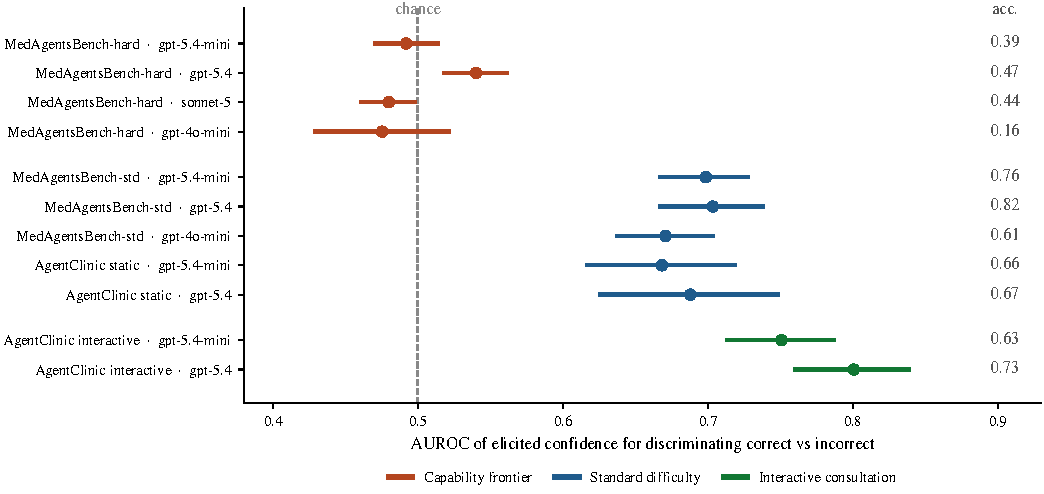
\includegraphics[width=0.92\textwidth]{figs/fig1_discrimination.pdf}
\caption{Discriminative power of elicited confidence, by deployment condition. Points are AUROC with
$95\%$ bootstrap intervals over episodes; the right-hand column gives task accuracy. The same model
spans chance to strong discrimination depending on condition: at the capability frontier confidence
is uninformative, on high-acuity presentations it is degraded beyond what difficulty predicts, and in
interactive consultation---where the model obtains its own evidence---it is most informative.}
\label{fig:disc}
\end{figure*}

\begin{table}[t]
\caption{Discrimination of elicited confidence across conditions. AUROC with $95\%$ bootstrap
interval; $\star$ indicates the interval excludes $0.5$.}
\label{tab:main}
\centering
\small
\resizebox{\columnwidth}{!}{%
\begin{tabular}{llrrl}
\toprule
Setting & Model & $n$ & Acc. & AUROC [95\% CI] \\
\midrule
\multicolumn{5}{l}{\emph{Clinical, static, capability frontier}}\\
MedAgentsBench-hard & gpt-5.4-mini & 2228 & .387 & .492 [.469, .515] \\
MedAgentsBench-hard & gpt-5.4 & 2235 & .474 & .540 [.517, .563]$^\star$ \\
MedAgentsBench-hard & sonnet-5 & 2948 & .445 & .480 [.460, .499] \\
MedAgentsBench-hard & gpt-4o-mini & 784 & .157 & .475 [.428, .523] \\
\multicolumn{5}{l}{\emph{Clinical, static, standard difficulty}}\\
MedAgentsBench-std & gpt-5.4-mini & 1198 & .760 & .699 [.666, .729]$^\star$ \\
MedAgentsBench-std & gpt-5.4 & 1200 & .824 & .703 [.666, .739]$^\star$ \\
MedAgentsBench-std & gpt-4o-mini & 800 & .613 & .671 [.637, .705]$^\star$ \\
AgentClinic (static) & gpt-5.4-mini & 409 & .655 & .669 [.617, .721]$^\star$ \\
AgentClinic (static) & gpt-5.4 & 303 & .667 & .689 [.628, .748]$^\star$ \\
\multicolumn{5}{l}{\emph{Clinical, high acuity}}\\
RedFlag-99 & gpt-5.4-mini & 594 & .581 & .617 [.575, .656]$^\star$ \\
RedFlag-99 & gpt-5.4 & 594 & .694 & .641 [.592, .688]$^\star$ \\
\multicolumn{5}{l}{\emph{Clinical, interactive consultation}}\\
AgentClinic (inter.) & gpt-5.4-mini & 642 & .632 & .751 [.713, .787]$^\star$ \\
AgentClinic (inter.) & gpt-5.4 & 642 & .727 & .800 [.759, .840]$^\star$ \\
\multicolumn{5}{l}{\emph{Non-clinical controls}}\\
MMLU-Pro & gpt-5.4-mini & 600 & .742 & .704 [.659, .747]$^\star$ \\
ARC-Challenge & gpt-5.4-mini & 600 & .958 & .782 [.683, .874]$^\star$ \\
MedCalc & gpt-5.4-mini & 581 & .690 & .693 [.650, .736]$^\star$ \\
GSM8K & gpt-5.4-mini & 599 & .846 & .534 [.505, .566]$^\star$ \\
\bottomrule
\end{tabular}}
\end{table}


\begin{table}[t]
\caption{Per-source decomposition, \texttt{gpt-5.4-mini}. Under the standard split no source falls
below chance; under the hard split four of ten do. The collapse is a property of the difficulty
stratum rather than of any particular source.}
\label{tab:source}
\centering
\small
\resizebox{\columnwidth}{!}{%
\begin{tabular}{lrrrrr}
\toprule
& \multicolumn{2}{c}{Capability frontier} & \multicolumn{2}{c}{Standard difficulty} \\
\cmidrule(lr){2-3}\cmidrule(lr){4-5}
Source & Acc. & AUROC & Acc. & AUROC \\
\midrule
AfriMedQA & .354 & \textbf{.319} & .783 & .518 \\
MedExQA & .237 & \textbf{.410} & .858 & .588 \\
PubMedQA & .153 & \textbf{.368} & .672 & .700 \\
MedXpertQA-U & .310 & \textbf{.455} & .375 & .569 \\
MMLU & .461 & .504 & .958 & .841 \\
MedXpertQA-R & .296 & .504 & .504 & .557 \\
MMLU-Pro & .400 & .529 & .817 & .842 \\
MedMCQA & .397 & .550 & .875 & .802 \\
MedBullets & .573 & .596 & .800 & .720 \\
MedQA & .671 & .625 & .950 & .577 \\
\bottomrule
\end{tabular}}
\end{table}

\begin{table}[t]
\caption{RedFlag-99 annotation. Three independent automated annotators; no physician review.
Principal analyses are repeated on the unanimous subset (Section~V-D).}
\label{tab:annot}
\centering
\small
\begin{tabular}{lrr}
\toprule
Agreement & Items & Share \\
\midrule
3 of 3 annotators & 77 & 77.8\% \\
2 of 3 & 11 & 11.1\% \\
1 of 3 & 6 & 6.1\% \\
0 of 3 & 5 & 5.1\% \\
\midrule
\multicolumn{3}{l}{Fleiss' $\kappa = 0.487$; mean self-rated clarity $4.26/5$}\\
\bottomrule
\end{tabular}
\end{table}

\subsection{The pattern holds on independent corpora}
Table~\ref{tab:source} decomposes the two clinical strata by source. Under the standard
split no source falls below chance. Under the hard split four of ten do---AfriMedQA at $0.319$,
PubMedQA at $0.368$, MedExQA at $0.410$, MedXpertQA-U at $0.455$---so on those sources stated
confidence is not merely uninformative but inverted: the answers the model is more confident about
are, if anything, more often wrong. The two sources retaining the most discrimination at the
frontier, MedQA and MedBullets, are also the two on which the model is most accurate there,
consistent with the association reported above.

The clinical sets share a benchmark family, so the standard-versus-frontier contrast could reflect a
property of that construction. Three independent corpora reproduce the association between
competence and discrimination: MMLU-Pro at accuracy $0.742$ gives $0.704$ $[0.659,0.747]$,
ARC-Challenge at $0.958$ gives $0.782$ $[0.683,0.874]$, and the free-response MedCalc set at $0.690$
gives $0.693$ $[0.650,0.736]$. Answer format is not the operative variable: MedCalc is numeric
free-response and behaves like the multiple-choice sets. Fig.~\ref{fig:trend} places all nine sets on
common axes; the association between competence and discrimination is visible, as are the two
systematic departures from it that this paper is about---RedFlag-99 below the trend and interactive
consultation above it.

One control is an outlier. GSM8K combines high accuracy ($0.846$) with near-chance discrimination
($0.534$ $[0.505,0.566]$). We tested and rejected two accounts of it in Section~VI-A. Because it is
the only set on which the association fails, we report the association as robust but not exceptionless.


\begin{table}[t]
\caption{First stage: realised reasoning tokens by assigned operating point,
\texttt{gpt-5.4-mini}. The assignment moves the resource by more than an order of magnitude with no
truncation, which is what licenses treating the nominal effort setting as a resource manipulation
rather than a label.}
\label{tab:firststage}
\centering
\small
\begin{tabular}{lrrrrr}
\toprule
Operating point & $n$ & Median & IQR & p90 & Trunc. \\
\midrule
\texttt{high} & 745 & 688 & [284, 1846] & 3375 & .000 \\
\texttt{low} & 745 & 80 & [42, 159] & 317 & .000 \\
\texttt{none} & 745 & 0 & [0, 0] & 0 & .000 \\
\bottomrule
\end{tabular}
\end{table}

\begin{table}[t]
\caption{Threats to validity and the design element that addresses each. Every row is a control run
rather than an argument; the section giving the result is named.}
\label{tab:threats}
\centering
\small
\resizebox{\columnwidth}{!}{%
\begin{tabular}{lll}
\toprule
Threat & Control & Result \\
\midrule
Class balance & accuracy-matched resampling \eqref{eq:match} & V-C: unchanged \\
Response format & four elicitation formats & V-C: all at chance \\
Response scale & 1--5 vs 1--10 vs 1--100 & V-H: no signal created \\
Elicitation position & confidence before vs after answer & V-H: unchanged \\
Differential cap & $K \in \{3,5,10\}$ & V-H: breadth only \\
Poor verbalisation & sampling self-consistency & V-C: no better \\
Ceiling censoring & escalation rule, per-episode log & IV-A: zero truncation \\
Corpus idiosyncrasy & three independent corpora & V-B: reproduces \\
Vendor & two vendors & V-A: reproduces \\
Architecture & non-reasoning model & V-A: reproduces \\
Item difficulty (acuity) & accuracy-matched controls & V-D: decrement persists \\
Annotation disagreement & unanimous-subset re-analysis & V-D: unchanged \\
\bottomrule
\end{tabular}}
\end{table}

\subsection{The frontier collapse is not a base-rate artifact}
Because accuracy differs between the standard and hard splits, the AUROC difference could in
principle reflect base rate rather than difficulty. Applying the matching of \eqref{eq:match} to the standard split leaves \eqref{eq:auc} unchanged: $0.698$ [$0.668$, $0.731$] at matched accuracy $0.387$, and
$0.703$ [$0.670$, $0.735$] at matched accuracy $0.474$, against unmatched values of $0.698$ and
$0.703$. The collapse is a property of the items, not of the class balance.

\subsection{No elicitation format recovers discrimination}
Across four formats and two operating points, all eight cells lie at chance: integer
$0.509$/$0.451$, probability $0.540$/$0.451$, verbal $0.486$/$0.490$, post-hoc self-check
$0.522$/$0.443$. Repeated sampling is likewise uninformative: within a fixed operating point,
self-consistency across three samples discriminates no better than the verbalized value
($0.500$--$0.562$ versus $0.527$--$0.563$). The failure is therefore not one of verbalization---there
is no accessible signal being poorly reported.

\subsection{Confidence degrades further on can't-miss presentations}
On RedFlag-99, AUROC is $0.617$ and $0.641$. Against accuracy-matched controls drawn from
standard-difficulty items, this is a decrement of $-0.082$ and $-0.063$, with the RedFlag value
falling outside the matched-control interval in both models
($0.699$ [$0.681$, $0.717$]; $0.704$ [$0.688$, $0.719$]). Fig.~\ref{fig:matched} shows the RedFlag value against the full matched-resample distribution.
Restricting to the 77 unanimously annotated items leaves the result unchanged ($0.619$ and $0.643$; decrements $-0.079$ and $-0.060$), so the
finding does not rest on items where annotators disagreed.


\begin{figure*}[t]
\centering
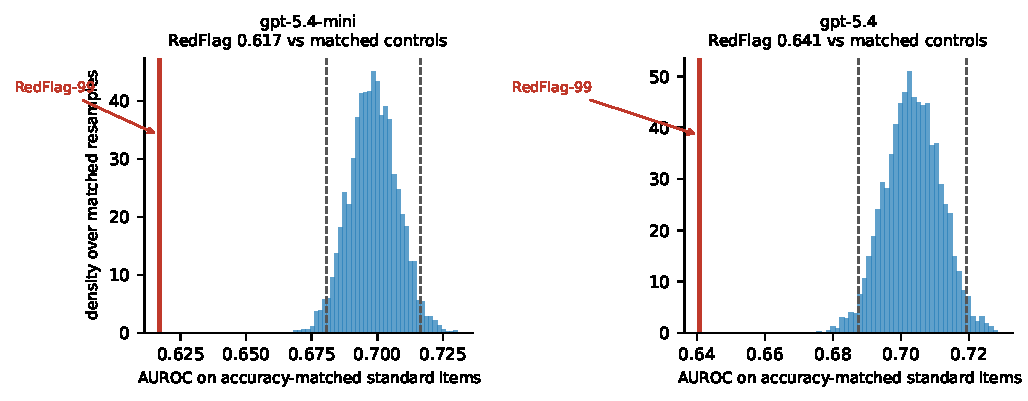
\includegraphics[width=0.92\textwidth]{figs/fig7_matched.pdf}
\caption{The high-acuity decrement is not a difficulty effect. Histograms give the distribution of
\eqref{eq:auc} over 3000 accuracy-matched resamples of standard-difficulty items drawn to the
accuracy of RedFlag-99 via \eqref{eq:match}; dashed lines mark the central $95\%$. The RedFlag value
(red) falls outside that interval for both models.}
\label{fig:matched}
\end{figure*}

\begin{figure}[t]
\centering
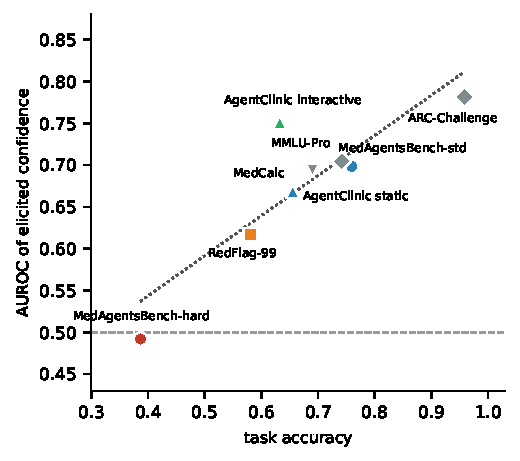
\includegraphics[width=\columnwidth]{figs/fig8_acc_vs_auc.pdf}
\caption{Discrimination against task accuracy across all nine evaluation sets,
\texttt{gpt-5.4-mini}. Competence and discrimination are associated (dotted trend), but the
association is not the whole story: RedFlag-99 sits below the trend, interactive consultation above
it, and GSM8K is an unexplained outlier at high accuracy and chance discrimination.}
\label{fig:trend}
\end{figure}

\subsection{Confidence does not predict the clinical endpoint}
A deferral gate serves two purposes usually conflated: catching wrong answers, and catching cases
where a time-critical diagnosis was never entertained. On RedFlag-99 these come apart. The
can't-miss condition appears in the elicited differential or the actively-excluded field in $92.1\%$
and $92.6\%$ of episodes, and confidence discriminates that endpoint at $0.687$ $[0.626,0.746]$ and
$0.667$ $[0.594,0.735]$---comparable to, and for the weaker model better than, its discrimination of
answer correctness on the same episodes ($0.617$, $0.641$). Deferral is correspondingly useful here:
evaluating \eqref{eq:dca}, routing the least-confident $22.4\%$ lowers the missed-red-flag rate from
$0.079$ to $0.056$ and from $0.074$ to $0.059$, and an aggressive threshold reduces it to $0.007$ (Table~\ref{tab:dca}).

The asymmetry is the finding. On the same items, elicited confidence carries usable information
about whether the dangerous diagnosis was considered while carrying degraded information about
whether the committed answer is right. A gate tuned on one endpoint does not serve the other.

\textbf{A construct caveat that bounds this result.} RedFlag-99 inherits its question stems from the
source benchmark, and those stems ask heterogeneous things: only $6$ of $99$ ask for the most likely
diagnosis, while $25$ ask for the next management step and $9$ for a causal organism. Where the stem
does not ask for a diagnosis, what the model enters in the differential field is shaped by the answer
options rather than being a clinical differential, so \eqref{eq:hit} is measured less directly there.
The high hit rate establishes that the can't-miss condition is usually present in the model's stated
reasoning, not that a differential-diagnostic exclusion was performed. A probe built from items that
uniformly ask for a diagnosis is the natural next step and is not available at usable scale from
existing benchmarks.

\begin{table}[t]
\caption{Decision-curve analysis on RedFlag-99. Deferral routes cases below the threshold to a
clinician; the endpoint is the missed-red-flag rate among cases retained for autonomous handling.}
\label{tab:dca}
\centering
\small
\resizebox{\columnwidth}{!}{%
\begin{tabular}{llrrr}
\toprule
Model & Threshold & Deferred & Missed rate & $\Delta$ vs.\ none \\
\midrule
\multirow{4}{*}{gpt-5.4-mini}
 & none & 0.0\% & .079 & --- \\
 & $\geq 8$ & 4.0\% & .077 & $-.002$ \\
 & $\geq 9$ & 22.4\% & .056 & $-.023$ \\
 & $\geq 10$ & 74.4\% & .007 & $-.073$ \\
\midrule
\multirow{4}{*}{gpt-5.4}
 & none & 0.0\% & .074 & --- \\
 & $\geq 8$ & 6.4\% & .070 & $-.004$ \\
 & $\geq 9$ & 22.4\% & .059 & $-.016$ \\
 & $\geq 10$ & 59.1\% & .025 & $-.049$ \\
\bottomrule
\end{tabular}}
\end{table}

\begin{figure*}[t]
\centering
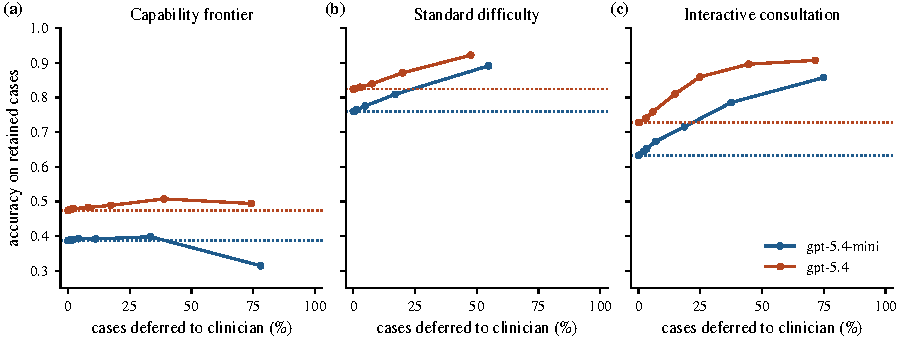
\includegraphics[width=0.92\textwidth]{figs/fig2_decision_curves.pdf}
\caption{Decision curves for confidence-gated deferral. Left: high-acuity static cases, endpoint
``can't-miss diagnosis considered''. Right: interactive consultation, endpoint diagnostic accuracy.
Dotted lines mark the no-deferral baseline. Note the order-of-magnitude difference in vertical
scale: on high-acuity cases deferral buys a few points and, for the weaker model, becomes harmful
beyond $60\%$ deferral; in interactive consultation the same mechanism on the same case material
yields large, monotone gains.}
\label{fig:dca}
\end{figure*}

\subsection{Interactive consultation restores discrimination}
On the same 214 AgentClinic cases, presented interactively rather than as complete vignettes,
confidence discriminates at $0.751$ [$0.713$, $0.787$] and $0.800$ [$0.759$, $0.840$], against
$0.669$ and $0.689$ for the static presentation of the same cases. Table~\ref{tab:intvsstatic} places the two presentations side by side. Deferral becomes useful:
routing the least-confident $18.5\%$ raises accuracy of the retained set from $0.632$ to $0.715$, and
routing $37.5\%$ raises it to $0.786$ (Fig.~\ref{fig:dca}, right; Table~\ref{tab:inter}). The stronger model shows the same
pattern, from $0.727$ to $0.859$ at $24.8\%$ deferral.

\begin{table}[t]
\caption{Deferral value in interactive consultation, AgentClinic (214 cases $\times$ 3 seeds).}
\label{tab:inter}
\centering
\small
\resizebox{\columnwidth}{!}{%
\begin{tabular}{llrrr}
\toprule
Model & Threshold & Deferred & Acc.\ retained & $\Delta$ \\
\midrule
\multirow{4}{*}{gpt-5.4-mini}
 & none & 0.0\% & .632 & --- \\
 & $\geq 8$ & 18.5\% & .715 & $+.083$ \\
 & $\geq 9$ & 37.5\% & .786 & $+.153$ \\
 & $\geq 10$ & 74.9\% & .857 & $+.225$ \\
\midrule
\multirow{4}{*}{gpt-5.4}
 & none & 0.0\% & .727 & --- \\
 & $\geq 8$ & 24.8\% & .859 & $+.132$ \\
 & $\geq 9$ & 44.5\% & .896 & $+.169$ \\
 & $\geq 10$ & 71.5\% & .907 & $+.180$ \\
\bottomrule
\end{tabular}}
\end{table}


\begin{figure*}[t]
\centering
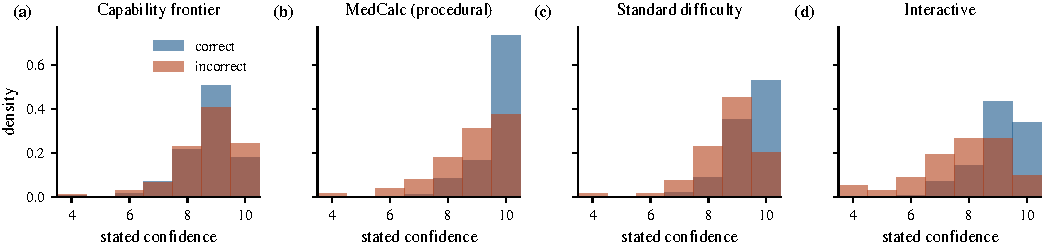
\includegraphics[width=0.96\textwidth]{figs/fig3_distributions.pdf}
\caption{Distribution of stated confidence for correct (blue) and incorrect (red) episodes,
\texttt{gpt-5.4-mini}. At the capability frontier the two distributions are superimposed; separation
appears at standard difficulty and is widest under interactive consultation.}
\label{fig:dist}
\end{figure*}

\begin{figure*}[t]
\centering
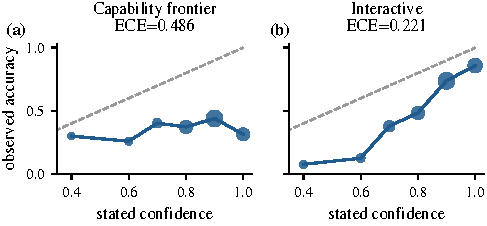
\includegraphics[width=0.96\textwidth]{figs/fig4_reliability.pdf}
\caption{Reliability diagrams, \texttt{gpt-5.4-mini}; marker area is proportional to bin occupancy
and the dashed line is perfect calibration. At the capability frontier the curve is essentially
flat---observed accuracy is unrelated to stated confidence over its whole range---whereas the
interactive curve is monotone. Expected calibration error is reported above each panel, and moves in
the same direction as discrimination without being equivalent to it.}
\label{fig:rel}
\end{figure*}

\begin{figure}[t]
\centering
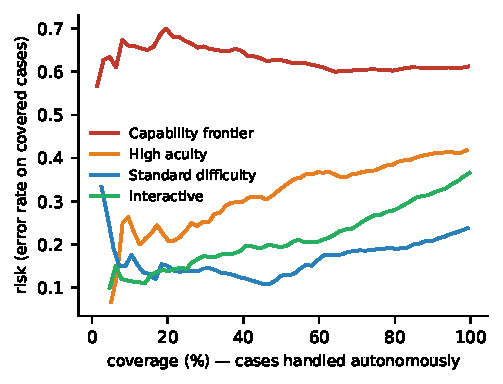
\includegraphics[width=\columnwidth]{figs/fig5_risk_coverage.pdf}
\caption{Risk--coverage curves. Cases are handled autonomously in decreasing order of stated
confidence. A useful confidence signal produces a curve rising steeply to the left; the
capability-frontier and high-acuity curves are nearly flat.}
\label{fig:rc}
\end{figure}

\begin{figure*}[t]
\centering
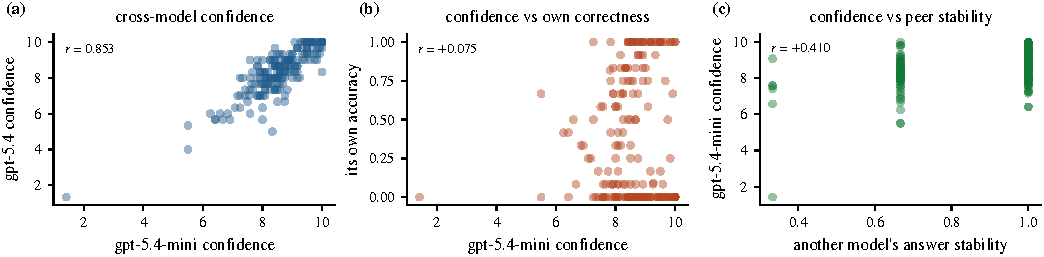
\includegraphics[width=0.96\textwidth]{figs/fig6_mechanism.pdf}
\caption{What elicited confidence tracks. Left: two models from different vendors agree strongly on
which items warrant confidence. Centre: neither model's confidence predicts its own correctness.
Right: a model's confidence is predicted about as well by \emph{another} model's answer stability as
by its own, which excludes within-episode circularity.}
\label{fig:mech}
\end{figure*}

\subsection{Sensitivity to elicitation design}
Three aspects of the elicitation schema could in principle drive the results: the cap on the
elicited differential, the position of the confidence field relative to the answer, and the
granularity of the confidence scale. Table~\ref{tab:abl} reports each.

Varying the differential cap $K \in \{3,5,10\}$ moves elicited breadth as intended
($2.91 \to 3.82 \to 4.15$ at standard difficulty) while leaving discrimination unchanged
($0.690$, $0.682$, $0.724$; all intervals overlapping), and the frontier condition is likewise
unmoved ($0.490$, $0.498$, $0.507$). The schema's ceiling therefore governs how much the model
lists, not how well its confidence separates correct from incorrect answers---which also means the
breadth measure and the discrimination measure are not two views of one quantity.

Moving the confidence field ahead of the answer, so that the model commits to a confidence before
committing to a response, changes nothing at standard difficulty ($0.692$ versus $0.682$) and if
anything weakens the frontier condition further ($0.447$ versus $0.496$, intervals overlapping).
Joint generation of answer and confidence is therefore not what produces the null: a confidence
stated before the answer exists is no more informative than one stated after.

Coarsening the response scale from ten levels to five costs discrimination at standard difficulty
($0.764 \to 0.642$) without changing the frontier condition ($0.477$ versus $0.499$, overlapping).
The scale therefore limits how finely a usable signal can be expressed but does not create one where
none exists---which is the expected pattern if the constraint is on the information available rather
than on the channel carrying it.


\begin{table}[t]
\caption{Sensitivity to elicitation design, \texttt{gpt-5.4-mini}, 150 items per split.
Varying the differential cap changes elicited breadth but not discrimination; presenting the
confidence field before the answer does not change it either. Neither aspect of the schema is
load-bearing.}
\label{tab:abl}
\centering
\small
\resizebox{\columnwidth}{!}{%
\begin{tabular}{llrrrl}
\toprule
Ablation & Variant & Acc. & Breadth & AUROC & [95\% CI] \\
\midrule
\multicolumn{6}{l}{\emph{Standard difficulty}}\\
\multirow{3}{*}{Differential cap $K$}
 & $K=3$ & .767 & 2.91 & .690 & [.624, .751] \\
 & $K=5$ (default) & .766 & 3.82 & .682 & [.617, .745] \\
 & $K=10$ & .747 & 4.15 & .724 & [.662, .785] \\
\multirow{2}{*}{Confidence position}
 & after answer (default) & .766 & 3.82 & .682 & [.615, .745] \\
 & before answer & .755 & 3.78 & .692 & [.627, .754] \\
\multirow{2}{*}{Confidence scale}
 & 1--5 & .750 & --- & .642 & [.573, .709] \\
 & 1--10 (default) & .773 & --- & .764 & [.703, .820] \\
\midrule
\multicolumn{6}{l}{\emph{Capability frontier}}\\
\multirow{3}{*}{Differential cap $K$}
 & $K=3$ & .339 & 2.91 & .490 & [.427, .553] \\
 & $K=5$ (default) & .353 & 3.88 & .498 & [.437, .561] \\
 & $K=10$ & .367 & 4.31 & .507 & [.446, .570] \\
\multirow{2}{*}{Confidence position}
 & after answer (default) & .353 & 3.88 & .496 & [.435, .559] \\
 & before answer & .380 & 3.84 & .447 & [.385, .510] \\
\multirow{2}{*}{Confidence scale}
 & 1--5 & .347 & --- & .499 & [.437, .560] \\
 & 1--10 (default) & .363 & --- & .477 & [.415, .539] \\
\bottomrule
\end{tabular}}
\end{table}


\begin{table}[t]
\caption{Cost of transferring a deferral threshold across conditions. The threshold is the smallest
value achieving $\ge 0.85$ accuracy on the retained set in the calibration condition; it is then
applied unchanged in the deployment condition. Transfer into the high-acuity stratum fails from
every origin, and the failure is not detectable from the calibration condition.}
\label{tab:transfer}
\centering
\small
\resizebox{\columnwidth}{!}{%
\begin{tabular}{lllrrl}
\toprule
Model & Calibrated on & Deployed on & $\tau$ & Deferred & Acc.\ retained \\
\midrule
\multirow{4}{*}{gpt-5.4-mini}
 & standard bench & interactive & 10 & 74.9\% & .857 \\
 & standard bench & high acuity & 10 & 74.4\% & \textbf{.763} \\
 & static OSCE & high acuity & 10 & 74.4\% & \textbf{.763} \\
 & interactive & high acuity & 10 & 74.4\% & \textbf{.763} \\
\midrule
\multirow{3}{*}{gpt-5.4}
 & standard bench & interactive & 9 & 44.5\% & .896 \\
 & standard bench & high acuity & 9 & 22.4\% & \textbf{.759} \\
 & interactive & high acuity & 8 & 6.4\% & \textbf{.716} \\
\bottomrule
\end{tabular}}
\end{table}

\subsection{The cost of transferring a threshold}
The recommendation that a gate be validated where it will run is only useful if the cost of ignoring
it can be stated. We therefore calibrate a threshold in one condition and apply it unchanged in
another. Fixing a service level of $0.85$ accuracy on the retained set, Table~\ref{tab:transfer}
gives the smallest threshold meeting it in the calibration condition and the accuracy that threshold
actually delivers elsewhere.

Transfer into the high-acuity stratum fails from every origin tested. A threshold calibrated on
standard benchmark items, on static OSCE vignettes, or in interactive consultation delivers
$0.716$--$0.763$ on can't-miss presentations---between $9$ and $13$ points below the service level it
was chosen to guarantee---while still deferring up to three quarters of cases. The shortfall is
invisible from the calibration condition: the same threshold meets its target there, so nothing in
the validation data signals that it will not hold.

Transfer in the reverse direction is benign. A threshold calibrated on standard items exceeds its
target when applied to interactive consultation ($0.857$ and $0.896$), because discrimination is
better in that setting than where the threshold was set. The asymmetry matters operationally: the
direction of transfer that a development pipeline naturally takes---validate on a benchmark, deploy
to a harder stratum---is the direction that fails.

For \texttt{gpt-5.4-mini} no threshold reaches $0.85$ on high-acuity items at all; the calibration
procedure returns a degenerate threshold that defers every case. A gate calibrated on that stratum
therefore does not produce a conservative setting, it produces the abandonment of autonomy, which is
a different and more honest failure than silently under-performing.

\subsection{What elicited confidence tracks}
Fig.~\ref{fig:mech} summarises the three relationships. Confidence agrees across models more
strongly than accuracy does: mean pairwise correlation of
elicited confidence is $r=0.749$ across four models, against $r=0.646$ for correctness on the same
items. Within model, confidence correlates with the answer stability of \eqref{eq:stab} across
operating points ($r=0.36$--$0.50$), and---critically---predicts equally well from \emph{another}
model's answer stability ($r=0.30$--$0.34$), which rules out a within-episode circularity. Stability
itself carries little information about correctness ($r=0.05$--$0.13$). Confidence is therefore a
readout of answer convergence on an item, and convergence is only weakly related to being right.

\section{Discussion}

The practical conclusion is that ``is elicited confidence reliable?'' has no model-level answer. The
same model, on clinically similar material, spans chance to strong discrimination depending on
whether the item is at its capability frontier, whether it carries high clinical acuity, and whether
it gathered the evidence itself. Reporting a single calibration figure for a clinical LLM is
therefore not meaningful for deployment.

Two consequences follow for system design. First, confidence-gated deferral cannot be validated on
standard benchmark items and then deployed against high-acuity presentations: on exactly the cases
that motivate the safety mechanism, discrimination of answer correctness drops from $0.70$ to
$0.62$--$0.64$ even after difficulty is matched away. Second, and in the opposite direction, static benchmark evaluation \emph{understates}
confidence reliability for consultation agents. The interactive result is not a contradiction of the
static one: if confidence tracks answer convergence, then a model that has actively obtained the
discriminating finding converges for a reason, and its confidence inherits that reason. Evidence
acquisition supplies information that a fully-specified vignette never requires the model to earn.

That mechanism also explains why no elicitation format helps. All four formats read out the same
underlying convergence signal, so rewording the question cannot manufacture information that the
computation did not produce. It is consistent with general-domain findings that cross-model
confidence is dominated by a shared item factor~\cite{metacog2026} and that overconfidence stems
from insufficient conditioning on the model's own answer~\cite{advice2025}.

\subsection{Why the interactive result is not a contradiction}
The two headline findings---confidence fails at the frontier and on high-acuity cases, yet works in
interactive consultation---are reconciled by what confidence is tracking. If elicited confidence
reports convergence rather than correctness, its informativeness depends on whether convergence and
correctness happen to align in the setting at hand. On a fully specified vignette the model
converges or fails to converge for reasons largely independent of whether it is right: our data show
answer stability correlating with confidence at $r=0.36$--$0.50$ but with correctness at only
$r=0.05$--$0.13$. In interactive consultation the model that has obtained the discriminating finding
converges \emph{because} it obtained it, so convergence and correctness share a cause and confidence
inherits the information. Evidence acquisition thus supplies a signal that a complete vignette never
requires the model to earn.

This account also predicts the elicitation-format null. If the four formats read out the same
underlying convergence signal, rewording the question cannot manufacture information the computation
did not produce, and the ablations confirm that neither the response scale, the differential cap, nor
the position of the confidence field changes the outcome. It is consistent with general-domain
findings that cross-model confidence is dominated by a shared item factor~\cite{metacog2026} and that
overconfidence arises from insufficient conditioning on the model's own answer~\cite{advice2025}.

\subsection{Implications for clinical deployment}
Three consequences follow for systems that gate on confidence.

\emph{A gate must be validated in the modality it will run in.} Confidence measured on static
question sets underestimates its reliability for a consultation agent by roughly $0.08$ AUROC in our
data, and confidence measured in consultation would overstate reliability for a system that answers
from a completed record. Neither direction of extrapolation is safe, and the difference is larger
than the difference between the models we tested.

\emph{A gate must be validated on the acuity stratum it will protect}, and the cost of not doing so
is measurable. Table~\ref{tab:transfer} shows a threshold meeting a $0.85$ service level in
validation delivering $0.716$--$0.763$ on can't-miss presentations, with nothing in the validation
data to signal the shortfall. Validation on standard
benchmark items reports $0.70$; the same gate applied to can't-miss presentations delivers $0.62$ for
answer correctness. The endpoint of whether the can't-miss condition was entertained behaves
differently again, at $0.667$--$0.687$: the two endpoints a clinical gate must serve are not
interchangeable, and a deployment that measures one and assumes the other is protected has no basis
for that assumption.

\emph{Deferral thresholds must be chosen per endpoint, on a decision curve.} On RedFlag-99 the same
confidence signal supports aggressive gating for the missed-red-flag endpoint---deferring $74\%$
drives that rate from $0.079$ to $0.007$---while supporting it poorly for answer correctness. A
threshold chosen to optimise ECE, or a single threshold applied to both endpoints, cannot express
that difference, because the failure is in which cases are ranked highest rather than in the scale
on which they are ranked.

\subsection{Relation to prior findings}
Our general-domain observations---strong cross-model agreement in stated confidence, near-zero
within-model correlation with correctness, and no recovery from alternative elicitation---reproduce
what has been reported for non-clinical benchmarks~\cite{metacog2026,xiong2023}. We regard that
agreement as a validity check on our instrument rather than as a finding. The clinical results have
no counterpart in that literature because it does not stratify by clinical risk: the observation
that discrimination degrades further on can't-miss presentations, and collapses on the
missed-red-flag endpoint specifically, requires acuity labels and an endpoint separable from answer
correctness, both of which the RedFlag construction supplies.

\subsection{Limitations}
No physician reviewed the RedFlag-99 items; construct validity rests on a pre-registered mechanical
filter, automated annotation with reported reliability ($\kappa = 0.487$), and a sensitivity analysis
on the unanimous subset. RedFlag-99 draws disproportionately from one source benchmark. The
high-acuity condition was not evaluated interactively at adequate power, because only 13 of the 214
AgentClinic vignettes carry a can't-miss diagnosis; that cell is reported descriptively and should
not be over-read. Confidence was elicited jointly with the answer in a single response for the
principal conditions, which is the deployment-realistic protocol but confounds elicitation with
generation; the post-hoc format controls for this and shows no difference. One control dataset,
GSM8K, is an outlier that we cannot explain: accuracy is high ($0.846$) but discrimination is near
chance ($0.534$). We tested and rejected two accounts---answer format, since the free-response
MedCalc set discriminates normally ($0.693$), and error type, since confidence discriminates
execution slips and formula errors comparably (difference $+0.043$, CI $[-0.034, +0.119]$). A
reported confound in which reasoning models re-solve the problem when asked about
confidence~\cite{metacog2026} is a candidate we cannot test without access to reasoning traces.

\section{Conclusion}
Elicited confidence in clinical language models is not a stable property that can be measured once
and relied upon. Across 25{,}485 episodes, five models, two vendors and nine evaluation sets, its
discriminative power ranges from chance to strong within a single model, governed by whether the
item lies at the model's capability frontier, whether it carries a can't-miss presentation, and
whether the model gathered the evidence itself. The variation across conditions exceeds the variation
across models.

For deployment the operative findings are negative and specific. On presentations carrying
time-critical diagnoses, confidence discriminates answer correctness at $0.62$--$0.64$, below the
$0.70$ obtained on accuracy-matched standard items, while discriminating whether the can't-miss
diagnosis was considered at all at
$0.667$--$0.687$---the two endpoints a gate must serve do not degrade together, so no single
calibration figure describes both. Against this, the same models in interactive consultation reach
$0.75$--$0.80$ on answer correctness, and deferral there is genuinely useful.

The cost of ignoring this is quantified rather than asserted: a threshold meeting a $0.85$ service
level in validation returns $0.716$--$0.763$ when transferred to high-acuity cases, and the
development pipeline's natural direction of transfer---benchmark to deployment stratum---is the
failing one.

Confidence-gated deferral is therefore neither uniformly sound nor uniformly unsound. It should be
validated in the modality and on the acuity stratum in which it will operate, with a decision curve
rather than a calibration statistic, and a gate validated on standard benchmark questions should not
be assumed to protect high-acuity cases.

\section*{Data and Code Availability}
All benchmarks are publicly available. Episode-level records, the RedFlag-99 probe with its
construction pipeline and annotation, and analysis code are released with the paper.

\begin{thebibliography}{99}
\bibitem{agentclinic} S. Schmidgall \emph{et al.}, ``AgentClinic: a multimodal agent benchmark to evaluate AI in simulated clinical environments,'' \emph{npj Digital Medicine}, 2026.
\bibitem{kadavath2022} Saurav Kadavath \emph{et al.}, ``Language Models (Mostly) Know What They Know,'' \emph{arXiv:2207.05221}, 2022.
\bibitem{xiong2023} Miao Xiong \emph{et al.}, ``Can LLMs Express Their Uncertainty? An Empirical Evaluation of Confidence Elicitation in LLMs,'' \emph{arXiv:2306.13063}, 2023.
\bibitem{selfeval2023} Jiefeng Chen \emph{et al.}, ``Adaptation with Self-Evaluation to Improve Selective Prediction in LLMs,'' \emph{arXiv:2310.11689}, 2023.
\bibitem{selfcal2025} Chengsong Huang \emph{et al.}, ``Efficient Test-Time Scaling via Self-Calibration,'' \emph{arXiv:2503.00031}, 2025.
\bibitem{advice2025} Ki Jung Seo, Sehun Lim, Taeuk Kim, ``ADVICE: Answer-Dependent Verbalized Confidence Estimation,'' \emph{arXiv:2510.10913}, 2025.
\bibitem{distractor2025} Victor Wang, Elias Stengel-Eskin, ``Calibrating Verbalized Confidence with Self-Generated Distractors,'' \emph{arXiv:2509.25532}, 2025.
\bibitem{dca2025} Glenn Zhang \emph{et al.}, ``Direct Confidence Alignment: Aligning Verbalized Confidence with Internal Confidence In Large Language Models,'' \emph{arXiv:2512.11998}, 2025.
\bibitem{orce2026} Chen Li \emph{et al.}, ``ORCE: Order-Aware Alignment of Verbalized Confidence in Large Language Models,'' \emph{arXiv:2605.12446}, 2026.
\bibitem{latentconf2026} Ting-Yu Chen \emph{et al.}, ``Latent Confidence Alignment for LLM Self-Assessment,'' \emph{arXiv:2606.21937}, 2026.
\bibitem{overconf2026} Mario Sanz-Guerrero, Manuel Mager, Katharina von der Wense, ``Large Language Models Are Overconfident in Their Own Responses,'' \emph{arXiv:2606.03437}, 2026.
\bibitem{calsurvey2026} Noam Michael \emph{et al.}, ``Confidence Calibration in Large Language Models,'' \emph{arXiv:2605.23909}, 2026.
\bibitem{mirror2026} Jason Z Wang, ``MIRROR: A Hierarchical Benchmark for Metacognitive Calibration in Large Language Models,'' \emph{arXiv:2604.19809}, 2026.
\bibitem{metacog2026} M. Moran, Mark Whiting, ``LLMs Show No Signs Of Individuated Metacognition,'' \emph{arXiv:2605.24299}, 2026.
\bibitem{introspect2026} Atharv Naphade \emph{et al.}, ``Me, Myself, and $\pi$: Evaluating and Explaining LLM Introspection,'' \emph{arXiv:2603.20276}, 2026.
\bibitem{steermeta2026} Yanshi Li \emph{et al.}, ``Decomposing and Steering Functional Metacognition in Large Language Models,'' \emph{arXiv:2605.08942}, 2026.
\bibitem{actionbelief2025} Arka Pal \emph{et al.}, ``Knowing What You Know Is Not Enough: Large Language Model Confidences Don't Align With Their Actions,'' \emph{arXiv:2511.13240}, 2025.
\bibitem{trac2026} Dahai Yu \emph{et al.}, ``TrAC: Trace-Conditioned Answer Consistency for Efficient Uncertainty Quantification in LLMs,'' \emph{arXiv:2608.00422}, 2026.
\bibitem{conformal2026} Charafeddine Mouzouni, ``Black-Box Reliability Certification for AI Agents via Self-Consistency Sampling and Conformal Calibration,'' \emph{arXiv:2602.21368}, 2026.
\bibitem{cdur2026} Prakul Sunil Hiremath, Harshit R. Hiremath, ``Calibration Drift Under Reasoning: How Chain-of-Thought Budgets Induce Overconfidence in Large Language Models,'' \emph{arXiv:2606.11211}, 2026.
\bibitem{tokenprob2026} Avery Ma \emph{et al.}, ``From token probabilities to calibrated confidence: An empirical study of mathematical question answering,'' \emph{arXiv:2608.07827}, 2026.
\bibitem{sqlsel2026} Robert Richardson, ``What Predicts Correctness in Text-to-SQL? A Selective-Prediction Study,'' \emph{arXiv:2607.06799}, 2026.
\bibitem{medagents} Yanjun Shao \emph{et al.}, ``MedicalAgentsBench for Complex Medical Reasoning: Comparing Internalized Reasoning Models versus Externalized Agent-based Frameworks,'' \emph{Patterns}, 2025.
\bibitem{medcalc} Nikhil Khandekar \emph{et al.}, ``MedCalc-Bench: Evaluating Large Language Models for Medical Calculations,'' \emph{NeurIPS Datasets and Benchmarks}, 2024.
\bibitem{m1_2025} Xiaoke Huang \emph{et al.}, ``m1: Unleash the Potential of Test-Time Scaling for Medical Reasoning with Large Language Models,'' \emph{arXiv:2504.00869}, 2025.
\bibitem{ttsmed2025} Gyutaek Oh \emph{et al.}, ``Rethinking Test-Time Scaling for Medical AI: Model and Task-Aware Strategies for LLMs and VLMs,'' \emph{arXiv:2506.13102}, 2025.
\bibitem{thinkshift2026} Sai Adith Senthil Kumar, ``When Built-in Thinking Helps and Hurts: Constraint-Level Error Shifts in Instruction Following,'' \emph{arXiv:2606.09662}, 2026.
\bibitem{gastro2025} Nariman Naderi \emph{et al.}, ``Self-Reported Confidence of Large Language Models in Gastroenterology: Analysis of Commercial, Open-Source, and Quantized Models,'' \emph{arXiv:2503.18562}, 2025.
\bibitem{promptmed2025} Nariman Naderi \emph{et al.}, ``Evaluating Prompt Engineering Techniques for Accuracy and Confidence Elicitation in Medical LLMs,'' \emph{arXiv:2506.00072}, 2025.
\bibitem{safescale2026} Sebastian Wind \emph{et al.}, ``Safety and accuracy follow different scaling laws in clinical large language models,'' \emph{arXiv:2605.04039}, 2026.
\bibitem{infoseek2026} Krischan Braitsch \emph{et al.}, ``Information-seeking failures of large language models in agentic clinical reasoning,'' \emph{arXiv:2607.10275}, 2026.
\bibitem{residency2026} Valentin Liévin \emph{et al.}, ``ResidencyRL: Reinforcement Learning in Simulated Clinical Environments,'' \emph{arXiv:2608.07418}, 2026.
\bibitem{triage2026} Reza Khanmohammadi, Kundan Thind, Mohammad M. Ghassemi, ``Calibrated Triage, Not Autonomy: Confidence Estimation for Medical Vision-Language Models,'' \emph{arXiv:2606.15910}, 2026.
\bibitem{clinmm2026} Rui Yang \emph{et al.}, ``Evaluating Multi-Turn Multimodal Diagnostic Reasoning on Challenging Real-World Clinical Cases,'' \emph{arXiv:2607.25933}, 2026.
\bibitem{premature2026} Rebecca Handler, Suhana Bedi, Nigam Shah, ``Quantifying and Mitigating Premature Closure in Frontier LLMs,'' \emph{arXiv:2605.15000}, 2026.
\bibitem{drl2026} Jinsong Liu \emph{et al.}, ``Closing Reasoning Gaps in Clinical Agents with Differential Reasoning Learning,'' \emph{arXiv:2602.09945}, 2026.
\bibitem{ophtha2026} Ehsan Misaghi \emph{et al.}, ``Deliberative multi-agent large language models improve clinical reasoning in ophthalmology,'' \emph{arXiv:2603.21447}, 2026.
\bibitem{realicu2026} Chengzhi Shen \emph{et al.}, ``RealICU: Do LLM Agents Understand Long-Context ICU Data? A Benchmark Beyond Behavior Imitation,'' \emph{arXiv:2605.13542}, 2026.
\bibitem{deferedge2026} Amirmohammad Farzaneh, Osvaldo Simeone, ``Think Short, Defer Smart, Act, and Repeat: Calibrated Reasoning and Uncertainty-Aware Deferral for Edge LLM Agents,'' \emph{arXiv:2607.26865}, 2026.
\bibitem{fuelgauge2026} Yuedong Yang \emph{et al.}, ``Fuel Gauge: Estimating Chain-of-Thought Length Ahead of Time in Large Multimodal Models,'' \emph{arXiv:2603.10335}, 2026.
\bibitem{advdistill2026} Huizi Cui \emph{et al.}, ``Estimating the Black-box LLM Uncertainty with Distribution-Aligned Adversarial Distillation,'' \emph{arXiv:2605.05777}, 2026.
\bibitem{direag2026} Haorui Xu, Yuzhou Zhu, Liyuan Gao, ``DirEAG: Dirichlet Evidence Aggregation for Calibrating Verbalized Confidence in Mathematical Reasoning,'' \emph{arXiv:2608.20717}, 2026.
\bibitem{nova2026} Jiayu Liu \emph{et al.}, ``NOVA: NOise-aware Verbal Confidence CAlibration for Robust Large Language Models in RAG Systems,'' \emph{arXiv:2601.11004}, 2026.
\bibitem{semsamp2026} Zhanliang Wang \emph{et al.}, ``A Semantic-Sampling Framework for Evaluating Calibration in Open-Ended Question Answering,'' \emph{arXiv:2605.08432}, 2026.
\bibitem{codeunc2026} Yuling Shi \emph{et al.}, ``Code Is More Than Text: Uncertainty Estimation for Code Generation,'' \emph{arXiv:2606.09577}, 2026.
\bibitem{r1med2025} Birger Moell, Fredrik Sand Aronsson, Sanian Akbar, ``Medical Reasoning in LLMs: An In-Depth Analysis of DeepSeek R1,'' \emph{arXiv:2504.00016}, 2025.
\bibitem{scaffold2026} Fatma Betül Güreş \emph{et al.}, ``Structuring versus Problematizing: How LLM-based Agents Scaffold Learning in Diagnostic Reasoning,'' \emph{arXiv:2604.09158}, 2026.
\bibitem{grasp2026} Johannes Moll \emph{et al.}, ``GRASP: Gated Regression-Aware Skill Proposer for Self-Improving LLM Agents,'' \emph{arXiv:2605.29668}, 2026.
\end{thebibliography}

\end{document}
